% Provenance (never printed): cycle 4 SVT, "La planete Terre, l'environnement
% et l'action humaine": resources from the Earth, their geological origin, the
% time they take to form and the rate we use them; see
% sources/book1/PROVENANCE.md. Book 1, grade 9, chapter 3.
% Vocabulary guard: owns ore deposit (with concentration factor), aggregate,
% reserve. Resource, renewable resource, ore, raw material (chemistry grade
% 5), fossil fuels (chemistry grade 8) and element abundances (chemistry
% grade 9) are recalled in prose. Groundwater and aquifers are g6's. Coal,
% oil and gas are told, not defined: "source rock", "reservoir", "seal",
% "trap" and the coal ranks belong to Book 2 g11 (fossil-fuel-geology);
% "hydrothermal" is not used (later books). Scientific notation (grade 9).
\chapter{Os recursos da Terra}\label{ch:g9:earth-resources}

Um smartphone cabe no bolso, mas contém dezenas de elementos químicos:
cobre para os seus fios, neodímio para os ímãs do seu alto-falante, gálio
para a luz da sua tela, índio para a fina camada da tela que conduz a
eletricidade, e muitos outros. Cada um deles foi tirado do chão
em algum lugar da Terra. Uma casa contém muito mais: uma casa de família
média precisa de cerca de cem toneladas de \omterm{def:g3:stones-pebbles-sand:sand}{areia}, \omterm{def:g3:stones-pebbles-sand:pebble}{cascalho} e pedra
britada, e a sua parte das ruas e das escolas em volta, cerca de três
vezes mais. Em que lugar da Terra esses materiais são encontrados, e por
que ali?
% ledger: usgs:smartphone, usgs:aggregate (114 and 328 short tons: about 100 and 300 t)

\begin{recall}
Em química, você aprende que os materiais que tiramos da natureza são
\emph{recursos}; um \emph{minério} é uma \omterm{def:g3:stones-pebbles-sand:rock}{rocha} da qual se pode extrair um
metal; um recurso \emph{renovável} é renovado pela natureza tão depressa
quanto o usamos; o carvão, o petróleo e o gás natural são
\emph{combustíveis \omterm{def:g7:sediments-and-fossils:fossil}{fósseis}}; e o oxigênio, o silício, o alumínio e o ferro
são os elementos mais abundantes da \omterm{def:g6:inside-the-earth:layers}{crosta}. A \omterm{def:g6:water-underground:groundwater}{água subterrânea} enche os
\omterm{def:g6:water-underground:porosity}{poros} de um \omterm{def:g6:water-underground:aquifer}{aquífero}, e a \omterm{def:g4:clouds-rain-snow:precipitation}{chuva} o reabastece
(\cref{ch:g6:water-underground}). Os \omterm{def:g7:sediments-and-fossils:sediment}{sedimentos} se acumulam em camadas e
se tornam \omterm{def:g6:rocks-and-minerals:rock-families}{rochas sedimentares} (\cref{ch:g7:sediments-and-fossils}), em
tempos contados em milhões de anos (\cref{ch:g7:geological-time}).
\end{recall}

\section{Por que um metal precisa ser concentrado}

O cobre está em toda parte: uma \omterm{def:g3:stones-pebbles-sand:rock}{rocha} comum contém um pouco dele, alguns
gramas em cada cem quilogramas. Mas, para tirar um quilograma de cobre de
uma \omterm{def:g3:stones-pebbles-sand:rock}{rocha} assim, seria preciso escavar, triturar e tratar toneladas dela.
A mineração só compensa o custo onde a natureza reuniu o metal numa \omterm{def:g3:stones-pebbles-sand:rock}{rocha}
muito mais rica.
% ledger: perkins:ore-grades (copper 0.006 % of the crust)

\begin{definition}[Jazida e fator de concentração]\label{def:g9:earth-resources:ore-deposit}
Uma \emph{jazida}\index{jazida} é um corpo de \omterm{def:g3:stones-pebbles-sand:rock}{rocha} no qual processos
naturais concentraram um metal ou um \omterm{def:g6:rocks-and-minerals:mineral}{mineral} o bastante para que ele
possa ser extraído com lucro. O \emph{fator de
concentração}\index{fator de concentracao@fator de concentração} de um
metal é o número de vezes que o seu teor no minério é maior que o seu
teor médio na \omterm{def:g6:inside-the-earth:layers}{crosta}:
\[
\text{fator de concentração} = \frac{\text{teor no minério}}{\text{teor médio na crosta}} .
\]
\end{definition}
% ledger: perkins:ore-grades, earle:ore-grades

Os metais comuns da \omterm{def:g6:inside-the-earth:layers}{crosta}, o alumínio e o ferro, precisam ser
concentrados só cerca de quatro vezes. O cobre precisa de cerca de 80
vezes, o zinco de cerca de 600 vezes, e os metais mais raros do gráfico,
o ouro, o estanho e o cromo, de milhares de vezes. Quanto mais raro um
metal na \omterm{def:g6:inside-the-earth:layers}{crosta}, mais a natureza tem de trabalhar para fazer um minério
dele, e menos numerosos são os lugares onde ela fez isso.
% ledger: perkins:ore-grades, earle:ore-grades

\begin{example}[O cobre]
A \omterm{def:g6:inside-the-earth:layers}{crosta} contém em média \qty{0.006}{\%} de cobre; um minério de cobre
pode ser lavrado a partir de cerca de \qty{0.5}{\%}. O \omterm{def:g9:earth-resources:ore-deposit}{fator de
concentração} é $0.5 \div 0.006
\approx 83$, cerca de 80, ou perto de $10^2$. Outro livro didático adota
\qty{40}{ppm} (\qty{0.004}{\%}) para a \omterm{def:g3:stones-pebbles-sand:rock}{rocha} comum e \qty{1}{\%} para o
minério: $1 \div
0.004 = 250$. Os dois números diferem, mas os dois dizem a mesma coisa:
um minério de cobre é cerca de cem vezes mais rico que a \omterm{def:g3:stones-pebbles-sand:rock}{rocha} comum.
\end{example}
% ledger: perkins:ore-grades, earle:ore-grades

\begin{omfigure}
\begin{tikzpicture}
\begin{axis}[xbar, xmode=log, width=12cm, height=5.3cm, xmin=1, xmax=2e4,
  log origin=infty, bar width=9pt, enlarge y limits=0.1,
  ytick=data, yticklabels={alumínio, ferro, cobre, zinco, ouro, estanho, cromo},
  y dir=reverse, xlabel={fator de concentração (escala logarítmica)},
  xtick={1,10,100,1000,10000}, xticklabels={$1$,$10$,$10^2$,$10^3$,$10^4$},
  tick label style={font=\footnotesize}, label style={font=\small},
  nodes near coords, nodes near coords style={font=\scriptsize, anchor=west},
  point meta=explicit, xmajorgrids, grid style={black!12}]
\addplot[fill=omWarm!45, draw=omWarm!80!black] table[x=factor, y=x, meta=factor] {figdata/out/grade-9-concentration.dat};
\end{axis}
\end{tikzpicture}

{\small Quantas vezes a natureza tem de concentrar sete metais para fazer
um minério que valha a pena lavrar: o teor mínimo do minério dividido
pelo teor médio da \omterm{def:g6:inside-the-earth:layers}{crosta}. Cada passo da escala é dez vezes o anterior.
Dados: D.~Perkins e colaboradores, \emph{Mineralogy}, e, para o ouro,
S.~Earle, \emph{Environmental Geology}.}
% ledger: perkins:ore-grades, earle:ore-grades (figdata/grade-9/concentration.py)
\label{fig:g9:earth-resources:factors}
\end{omfigure}

\begin{method}[Calcular um fator de concentração]
\begin{enumerate}
  \item Escreva o teor do metal no minério e na \omterm{def:g6:inside-the-earth:layers}{crosta} média na mesma
        unidade (porcentagem, ou gramas por tonelada).
  \item Divida o teor no minério pelo teor na \omterm{def:g6:inside-the-earth:layers}{crosta}.
  \item Arredonde o resultado: o que importa é a sua ordem de grandeza,
        cerca de 10, 100 ou 1000, que você pode escrever como uma
        potência de dez.
\end{enumerate}
\end{method}


\section{Como as jazidas se formam}

A natureza concentra os metais de várias maneiras. Três delas aparecem abaixo.

\begin{omfigure}
\begin{tikzpicture}[x=1cm, y=1cm, font=\footnotesize, >={Stealth[length=2mm]}]
  % country rock
  \fill[black!13] (0,0) rectangle (13,4.6);
  % surface with a valley on the right
  \fill[white] (0,4.6) -- (8.4,4.6) -- (9.6,3.7) -- (11.2,3.7) -- (12.0,4.6) -- (13,4.6) -- (13,5.6) -- (0,5.6) -- cycle;
  \draw[black!60] (0,4.6) -- (8.4,4.6) -- (9.6,3.7) -- (11.2,3.7) -- (12.0,4.6) -- (13,4.6);
  % river gravels on the valley floor
  \fill[omLithCongl] (9.5,3.75) -- (11.3,3.75) -- (11.15,3.35) -- (9.65,3.35) -- cycle;
  \foreach \x in {9.8,10.1,10.45,10.8,11.05} \fill[black!45] (\x,3.6) circle (0.05);
  \foreach \x in {9.9,10.3,10.65,10.95} \fill[yellow!80!orange] (\x,3.4) circle (0.045);
  \fill[omRiver!60] (9.9,3.75) rectangle (10.9,3.85);
  % magma body (cooling granite)
  \fill[omLithGranite] (1.0,0) .. controls (1.2,1.6) and (2.2,2.1) .. (3.4,2.1)
     .. controls (4.6,2.1) and (5.6,1.6) .. (5.8,0) -- cycle;
  \draw[black!50] (1.0,0) .. controls (1.2,1.6) and (2.2,2.1) .. (3.4,2.1)
     .. controls (4.6,2.1) and (5.6,1.6) .. (5.8,0);
  % heavy minerals settled at the bottom of the magma body
  \fill[black!60] (1.05,0) rectangle (5.75,0.25);
  % cracks and veins above the magma
  \foreach \x/\a in {2.6/12, 3.4/-6, 4.3/-15} {
    \draw[black, line width=1.6pt] (\x,2.15) -- ++(90+\a:2.0);
    \draw[yellow!80!orange, line width=0.6pt] (\x,2.15) -- ++(90+\a:2.0);
  }
  % hot water rising
  \draw[->, omWarm, thick] (2.1,1.9) .. controls (1.9,2.7) and (2.2,3.2) .. (2.45,3.7);
  \draw[->, omWarm, thick] (4.95,1.7) .. controls (5.1,2.6) and (4.8,3.3) .. (4.55,3.8);
  % labels
  \node[anchor=north, align=center] at (3.4,1.35) {um corpo de magma que esfria};
  \node[anchor=west, align=left, fill=white, fill opacity=0.85, text opacity=1, inner sep=1.5pt] at (6.2,0.75)
    {\textbf{1} minerais pesados ricos em metal\\ se depositam no fundo};
  \draw[black!70] (6.15,0.65) -- (5.5,0.15);
  \node[anchor=west, align=left, fill=white, fill opacity=0.85, text opacity=1, inner sep=1.5pt] at (5.6,2.55)
    {\textbf{2} a água quente sobe pelas fendas,\\ esfria e deixa os metais: veios};
  \draw[black!70] (5.55,2.6) -- (4.2,3.3);
  \node[anchor=south, align=center] at (10.4,4.7) {\textbf{3} grãos de ouro se depositam com\\ o cascalho de um rio: um placer};
  \draw[black!70] (10.4,4.7) -- (10.3,3.45);
  \node[anchor=south west] at (0.1,4.65) {superfície do terreno};
\end{tikzpicture}

{\small Três maneiras de concentrar um metal (um esboço, fora de escala).
(1) Num corpo de \omterm{def:g7:volcanoes:magma}{magma}, \omterm{def:g6:rocks-and-minerals:mineral}{minerais} pesados ricos em níquel ou em cobre
afundam e se reúnem no fundo. (2) A \omterm{def:g6:water-underground:groundwater}{água subterrânea} aquecida pelo \omterm{def:g7:volcanoes:magma}{magma},
e a água liberada pelo próprio \omterm{def:g7:volcanoes:magma}{magma}, dissolvem metais, sobem pelas fendas
e os deixam onde a \omterm{def:g3:stones-pebbles-sand:rock}{rocha} é mais fria, enchendo as fendas de veios. (3) A
\omterm{def:g5:water-shapes-the-land:erosion}{erosão} liberta o ouro dos veios; o \omterm{def:g1:landscapes-around-us:water}{rio} o transporta, e os grãos pesados
se depositam entre os \omterm{def:g3:stones-pebbles-sand:pebble}{cascalhos}, até a \omterm{def:g3:stones-pebbles-sand:rock}{rocha} de base.}
% ledger: earle:magmatic, usgs:gold-lode, usgs:gold-placer
\label{fig:g9:earth-resources:deposits}
\end{omfigure}

\paragraph{No magma.} Quando um corpo de \omterm{def:g7:volcanoes:magma}{magma} esfria, os \omterm{def:g6:rocks-and-minerals:mineral}{minerais} que
se cristalizam primeiro nem sempre são os mais leves. Nos \omterm{def:g7:volcanoes:magma}{magmas} vindos
do \omterm{def:g6:inside-the-earth:layers}{manto}, \omterm{def:g6:rocks-and-minerals:mineral}{minerais} pesados ricos em níquel e em cobre afundam e se
reúnem numa camada rica. A maior parte do níquel lavrado no mundo vem de
\omterm{def:g9:earth-resources:ore-deposit}{jazidas} desse tipo.
% ledger: earle:magmatic

\paragraph{Nas fendas, pela água quente.} A \omterm{def:g6:water-underground:groundwater}{água subterrânea} que corre
perto de um corpo de \omterm{def:g7:volcanoes:magma}{magma}, a alguns quilômetros abaixo da superfície, é
aquecida e sobe pelas fendas da \omterm{def:g3:stones-pebbles-sand:rock}{rocha}. A água quente dissolve metais das
\omterm{def:g3:stones-pebbles-sand:rock}{rochas} que atravessa. Quando chega a uma \omterm{def:g3:stones-pebbles-sand:rock}{rocha} mais fria, mais perto da
superfície, os metais saem da água na forma de \omterm{def:g6:rocks-and-minerals:mineral}{minerais} e enchem as
fendas: são os \emph{veios}\index{veio}. Muitas \omterm{def:g9:earth-resources:ore-deposit}{jazidas} de ouro são
veios desse tipo. Em volta de alguns corpos de \omterm{def:g7:volcanoes:magma}{magma}, a água quente
atravessou toda uma massa de \omterm{def:g3:stones-pebbles-sand:rock}{rocha} fraturada e deixou cobre nela,
espalhado, mas num volume enorme: são as maiores \omterm{def:g9:earth-resources:ore-deposit}{jazidas} de cobre do
mundo.
% ledger: usgs:gold-lode, earle:porphyry

\begin{omfigure}
\begin{minipage}[c]{0.46\linewidth}\centering
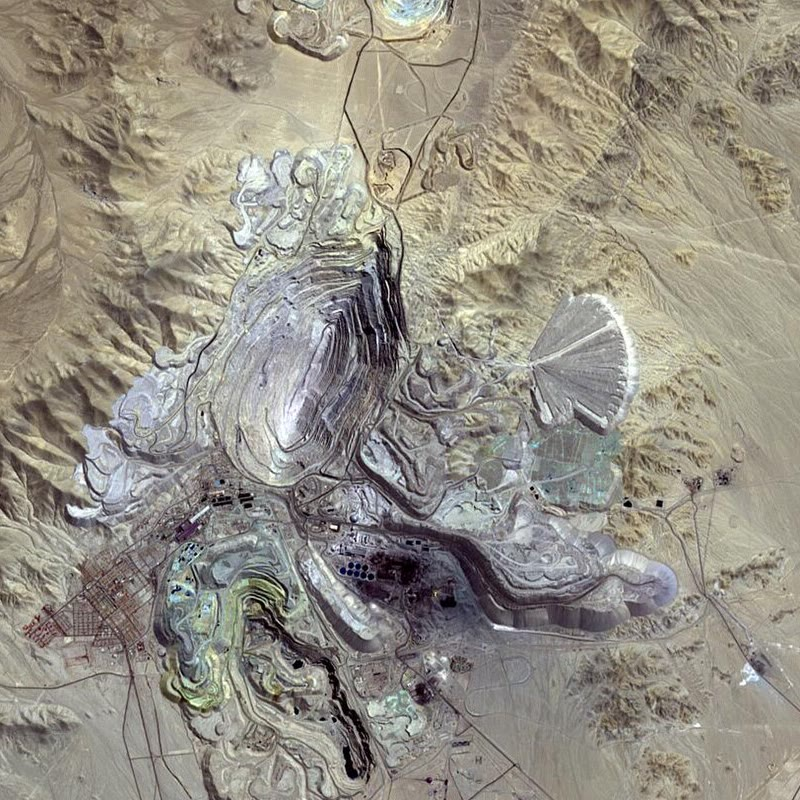
\includegraphics[width=\linewidth]{images/book1/g9-chuquicamata.jpg}
\end{minipage}\hfill
\begin{minipage}[c]{0.5\linewidth}\raggedright
{\small A mina de cobre de Chuquicamata, no \omterm{def:g5:weather-and-climate:desert}{deserto} do Atacama, no
Chile, vista pelo instrumento ASTER de um satélite da NASA em 2007 (a
imagem tem cerca de \qty{12}{km} de largura). A cava oval no meio,
explorada há mais de um século, tem \qty{4.3}{km} de comprimento,
\qty{2.7}{km} de largura e \qty{1.1}{km} de profundidade. NASA/METI/AIST/Japan
Space Systems e U.S./Japan ASTER Science Team (domínio público, via
Wikimedia Commons).}
\end{minipage}
% ledger: commons:chuquicamata, earle:chuquicamata
\label{fig:g9:earth-resources:chuquicamata}
\end{omfigure}

\paragraph{Nos cascalhos dos rios.} O ouro não enferruja e quase não
sofre \omterm{def:g5:water-shapes-the-land:weathering}{intemperismo}. Quando a \omterm{def:g5:water-shapes-the-land:erosion}{erosão} desgasta um veio de ouro, o ouro é
liberado como pó, palhetas, grãos e às vezes pepitas, e os \omterm{def:g1:landscapes-around-us:water}{rios} o levam
\omterm{def:g1:landscapes-around-us:water}{rio} abaixo. O ouro é muito denso: cerca de \qty{19}{g/cm^3} puro, contra
cerca de \qty{2.5}{g/cm^3} para a \omterm{def:g3:stones-pebbles-sand:rock}{rocha} comum. Nas cheias, quando todo o
leito de \omterm{def:g3:stones-pebbles-sand:sand}{areia} e \omterm{def:g3:stones-pebbles-sand:pebble}{cascalho} se move, os grãos pesados de ouro abrem
caminho para baixo e se acumulam sobre a \omterm{def:g3:stones-pebbles-sand:rock}{rocha} de base. Os geólogos
chamam esses depósitos de \emph{pláceres}\index{placer}.
% ledger: usgs:gold-placer

\section{Carvão, petróleo e gás}

O carvão, o petróleo e o gás natural são restos de seres vivos,
enterrados antes de poderem apodrecer. Quase toda a matéria orgânica de
uma planta ou de um animal morto volta a ser gás carbônico em algumas
semanas ou décadas. Só a parte isolada do oxigênio do ar, no fundo de um
pântano de água parada ou de um \omterm{def:g2:water-on-earth:ocean}{mar} profundo, pode ser enterrada e
conservada por milhões de anos.
% ledger: earle:coal, earle:oil-gas

\begin{omfigure}
\begin{minipage}[c]{0.46\linewidth}\centering
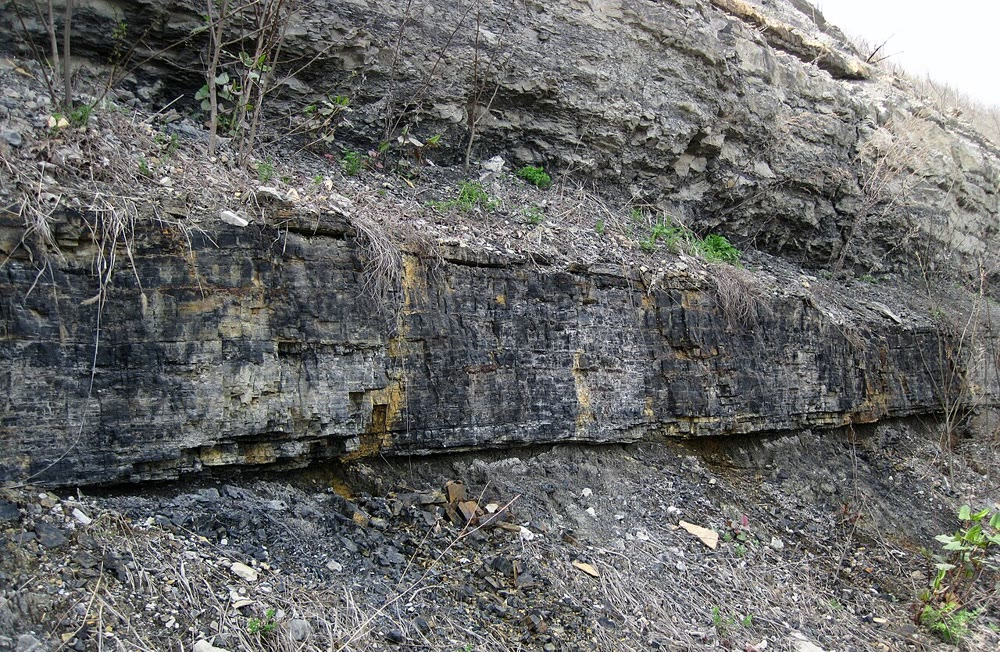
\includegraphics[width=\linewidth]{images/book1/g9-coal-seam.jpg}
\end{minipage}\hfill
\begin{minipage}[c]{0.5\linewidth}\raggedright
{\small Uma camada de carvão, a faixa escura no meio, entre \omterm{def:g6:rocks-and-minerals:rock-families}{rochas
sedimentares}, à beira de uma estrada em Ohio, nos Estados Unidos. A camada
é horizontal, como era o pântano. Fotografia de James St.~John (CC BY
2.0, via Wikimedia Commons).}
\end{minipage}
% ledger: commons:meigs-coal
\label{fig:g9:earth-resources:coal-seam}
\end{omfigure}


\paragraph{O carvão.} O carvão começa em pântanos ao lado de \omterm{def:g1:landscapes-around-us:water}{rios} e de
\omterm{def:g5:water-shapes-the-land:delta}{deltas}, em \omterm{def:g5:weather-and-climate:climate}{climas} quentes e úmidos, onde as plantas crescem depressa.
Troncos e folhas mortos caem numa água parada que contém pouco oxigênio,
e não apodrecem. O pântano tem de durar séculos ou milênios para formar
uma camada grossa. Um dia, um \omterm{def:g1:landscapes-around-us:water}{rio} muda de curso ou transborda e cobre o
pântano de \omterm{def:g3:stones-pebbles-sand:sand}{areia} e de \omterm{def:g3:stones-pebbles-sand:sand}{lama}. À medida que mais \omterm{def:g7:sediments-and-fossils:sediment}{sedimentos} se acumulam, a
camada de plantas é comprimida e aquecida, e se transforma em carvão:
primeiro um carvão marrom e macio, com cerca de um terço de carbono, a
algumas centenas de metros de profundidade; depois um carvão preto e
duro, com até 86~\% de carbono, a alguns quilômetros de profundidade. O
carvão lavrado hoje nos Estados Unidos, por exemplo, tem em sua maioria
de 100 a 300~milhões de anos.
% ledger: earle:coal, eia:coal

\begin{omfigure}
\begin{tikzpicture}[x=1cm, y=0.8cm, font=\footnotesize]
  \foreach \i/\t in {0/{(a) um pântano florestal:\\ plantas mortas se\\ acumulam na água parada},
                     1/{(b) enterrada sob areia\\ e lama do rio, a\\ camada é comprimida},
                     2/{(c) mais funda e quente\\ (centenas de metros):\\ carvão marrom e macio},
                     3/{(d) mais funda ainda\\ (quilômetros):\\ carvão preto e duro}} {
    \begin{scope}[xshift=\i*3.35cm]
      \draw[black!40] (0,0) rectangle (2.9,4.2);
      \node[align=center, anchor=north, font=\scriptsize] at (1.45,-0.1) {\t};
    \end{scope}
  }
  % (a) swamp: water, trees, plant layer
  \fill[omSea] (0,2.6) rectangle (2.9,3.1);
  \fill[brown!60!black!70] (0,2.0) rectangle (2.9,2.6);
  \fill[omLithShale] (0,0) rectangle (2.9,2.0);
  \foreach \x in {0.5,1.4,2.3} {
    \draw[brown!50!black, line width=1.2pt] (\x,2.6) -- (\x,3.7);
    \fill[green!45!black] (\x,3.85) circle (0.3);
  }
  % (b) buried
  \begin{scope}[xshift=3.35cm]
    \fill[lith sandstone] (0,2.6) rectangle (2.9,4.0);
    \fill[brown!55!black!80] (0,2.2) rectangle (2.9,2.6);
    \fill[omLithShale] (0,0) rectangle (2.9,2.2);
    \draw[->, thick] (1.45,4.15) -- (1.45,3.45);
  \end{scope}
  % (c) lignite
  \begin{scope}[xshift=6.7cm]
    \fill[lith sandstone] (0,1.9) rectangle (2.9,4.2);
    \fill[brown!45!black] (0,1.65) rectangle (2.9,1.9);
    \fill[omLithShale] (0,0) rectangle (2.9,1.65);
  \end{scope}
  % (d) coal
  \begin{scope}[xshift=10.05cm]
    \fill[lith sandstone] (0,1.25) rectangle (2.9,4.2);
    \fill[black!85] (0,1.1) rectangle (2.9,1.25);
    \fill[omLithShale] (0,0) rectangle (2.9,1.1);
  \end{scope}
\end{tikzpicture}

{\small De um pântano a uma camada de carvão (um esboço, fora de escala).
À medida que a camada de plantas afunda, ela é comprimida e aquecida: a
água e os gases saem dela, ela fica mais fina, e a sua parte de carbono
aumenta.}
% ledger: earle:coal, eia:coal
\label{fig:g9:earth-resources:coal}
\end{omfigure}


\paragraph{O petróleo e o gás.} O petróleo e a maior parte do gás
natural vêm das minúsculas plantas e dos minúsculos animais que vivem no
\omterm{def:g2:water-on-earth:ocean}{mar}, como as diatomáceas. Os seus restos afundam com a \omterm{def:g3:stones-pebbles-sand:sand}{lama} até o fundo
do \omterm{def:g2:water-on-earth:ocean}{mar}, e alguns são enterrados antes de se decompor. Milhões de anos e
quilômetros de \omterm{def:g7:sediments-and-fossils:sediment}{sedimentos} depois, o calor e a pressão os transformam:
abaixo de cerca de \qty{2}{km}, entre cerca de 60 e
\qty{120}{\degreeCelsius}, em petróleo; ainda mais quente, em gás. O
petróleo e o gás são mais leves que a água. Eles sobem devagar pelos
\omterm{def:g6:water-underground:porosity}{poros} das \omterm{def:g3:stones-pebbles-sand:rock}{rochas} \omterm{def:g6:water-underground:permeability}{permeáveis}, e muitos chegam à superfície e se perdem. Os
que encontramos foram parados no caminho por uma camada de \omterm{def:g3:stones-pebbles-sand:rock}{rocha}
\omterm{def:g6:water-underground:permeability}{impermeável}, muitas vezes no alto de uma dobra arqueada para cima, onde
se acumulam: o gás no alto, o petróleo embaixo dele e a água por baixo.
% ledger: eia:oil, eia:gas, earle:oil-gas

\begin{omfigure}
\begin{tikzpicture}[x=1cm, y=1cm, font=\footnotesize, >={Stealth[length=2mm]}]
  \def\fold#1{(0,#1) .. controls (3,#1+1.0) and (4.0,#1+1.6) .. (6,#1+1.6) .. controls (8.0,#1+1.6) and (9,#1+1.0) .. (12,#1)}
  % layers from the bottom up
  \fill[omLithShale!60!black!40] (0,0) -- \fold{0.9} -- (12,0) -- cycle;
  \fill[lith sandstone] \fold{0.9} -- (12,2.1) -- (12,2.1) .. controls (9,3.1) and (8.0,3.7) .. (6,3.7) .. controls (4.0,3.7) and (3,3.1) .. (0,2.1) -- cycle;
  \fill[lith shale] (0,2.1) .. controls (3,3.1) and (4.0,3.7) .. (6,3.7) .. controls (8.0,3.7) and (9,3.1) .. (12,2.1) -- (12,3.6) .. controls (9,4.6) and (8.0,5.2) .. (6,5.2) .. controls (4.0,5.2) and (3,4.6) .. (0,3.6) -- cycle;
  \fill[lith sandstone] (0,3.6) .. controls (3,4.6) and (4.0,5.2) .. (6,5.2) .. controls (8.0,5.2) and (9,4.6) .. (12,3.6) -- (12,5.6) -- (0,5.6) -- cycle;
  % gas and oil under the crest of the impermeable layer
  \fill[omWxSun!60] (4.55,3.55) .. controls (5.2,3.69) and (6.8,3.69) .. (7.45,3.55) -- (7.1,3.35) -- (4.9,3.35) -- cycle;
  \fill[black!75] (4.9,3.35) -- (7.1,3.35) -- (8.05,3.05) .. controls (7.0,3.15) and (5.0,3.15) .. (3.95,3.05) -- cycle;
  % arrows: oil creeping up through the permeable layer
  \draw[->, black, thick] (1.4,2.05) -- (2.4,2.55);
  \draw[->, black, thick] (10.6,2.05) -- (9.6,2.55);
  \draw[->, black!70] (3.0,2.65) -- (3.8,2.95);
  \draw[->, black!70] (9.0,2.65) -- (8.2,2.95);
  % labels
  \node[anchor=west, fill=white, fill opacity=0.85, text opacity=1, inner sep=1.5pt] at (0.1,0.45) {lama escura do antigo fundo do mar: aqui se formam o petróleo e o gás};
  \node[anchor=east, fill=white, fill opacity=0.85, text opacity=1, inner sep=1.5pt] at (11.9,1.9) {arenito permeável};
  \node[anchor=east, fill=white, fill opacity=0.85, text opacity=1, inner sep=1.5pt] at (11.9,3.25) {folhelho impermeável};
  \node[anchor=south, fill=white, fill opacity=0.85, text opacity=1, inner sep=1.5pt] at (6,5.25) {rochas da superfície};
  \node[font=\scriptsize] at (6,3.48) {gás};
  \node[font=\scriptsize, text=white] at (6,3.22) {petróleo};
\end{tikzpicture}

{\small O petróleo e o gás parados sob uma camada \omterm{def:g6:water-underground:permeability}{impermeável} no alto de
uma dobra arqueada para cima (um esboço, fora de escala; a água que enche
o resto do arenito não está representada). Abaixo da dobra, eles sobem
pelo arenito \omterm{def:g6:water-underground:permeability}{permeável} (setas) e se acumulam sob a crista: o gás em cima,
o petróleo embaixo.}
% ledger: earle:oil-gas
\label{fig:g9:earth-resources:oil}
\end{omfigure}

\section{A água do subsolo}

A \omterm{def:g6:water-underground:groundwater}{água subterrânea} também é um recurso da Terra, aquele que usamos todos
os dias. Ao contrário de um metal ou do carvão, ela se renova: a \omterm{def:g4:clouds-rain-snow:precipitation}{chuva}
reabastece os \omterm{def:g6:water-underground:aquifer}{aquíferos}. Mas ela se renova devagar, e só tão depressa
quanto a \omterm{def:g4:clouds-rain-snow:precipitation}{chuva} se infiltra. Um \omterm{def:g6:water-underground:aquifer}{aquífero} bombeado mais depressa do que é
reabastecido vê o seu \omterm{def:g6:water-underground:water-table}{lençol freático} baixar, e os \omterm{def:g6:water-underground:spring}{poços} secam
(\cref{ch:g6:water-underground}). A \omterm{def:g6:water-underground:groundwater}{água subterrânea} só é um recurso
renovável enquanto não for retirada mais depressa do que se renova.
% ledger: wss:aquifer

\section{A areia e o cascalho}

O material sólido que as pessoas tiram do chão nas maiores quantidades
não é nem o carvão nem um minério de metal: é a \omterm{def:g3:stones-pebbles-sand:sand}{areia} e o \omterm{def:g3:stones-pebbles-sand:pebble}{cascalho}.
% ledger: tos:sand

\begin{definition}[Agregado]\label{def:g9:earth-resources:aggregate}
Os \emph{agregados}\index{agregado} são a \omterm{def:g3:stones-pebbles-sand:sand}{areia}, o \omterm{def:g3:stones-pebbles-sand:pebble}{cascalho} e a pedra
britada usados na construção: no concreto, embaixo de estradas e de
ferrovias, e para aterrar o terreno.
\end{definition}
% ledger: usgs:aggregate, tos:sand

A maior parte da \omterm{def:g3:stones-pebbles-sand:sand}{areia} vai para o concreto, uma mistura de \omterm{def:g3:stones-pebbles-sand:sand}{areia},
\omterm{def:g3:stones-pebbles-sand:pebble}{cascalho}, água e cimento. Em 2019, o mundo precisava de cerca de
50~bilhões de toneladas de \omterm{def:g3:stones-pebbles-sand:sand}{areia} e \omterm{def:g3:stones-pebbles-sand:pebble}{cascalho} por ano, ou seja,
$5 \times 10^{10}$ toneladas, ou cerca de \qty{18}{kg} para cada pessoa
da Terra, todos os dias. A \omterm{def:g3:stones-pebbles-sand:sand}{areia} e o \omterm{def:g3:stones-pebbles-sand:pebble}{cascalho} são extraídos de cavas em
terra, de leitos de \omterm{def:g1:landscapes-around-us:water}{rios} e, cada vez mais, do fundo do \omterm{def:g2:water-on-earth:ocean}{mar}. Tirados de
um \omterm{def:g1:landscapes-around-us:water}{rio}, eles deixam menos \omterm{def:g3:stones-pebbles-sand:sand}{areia} chegar ao \omterm{def:g1:landscapes-around-us:water}{litoral}, e as praias \omterm{def:g1:landscapes-around-us:water}{rio} abaixo
se desgastam.
% ledger: tos:sand

\begin{omfigure}
\begin{minipage}[c]{0.46\linewidth}\centering
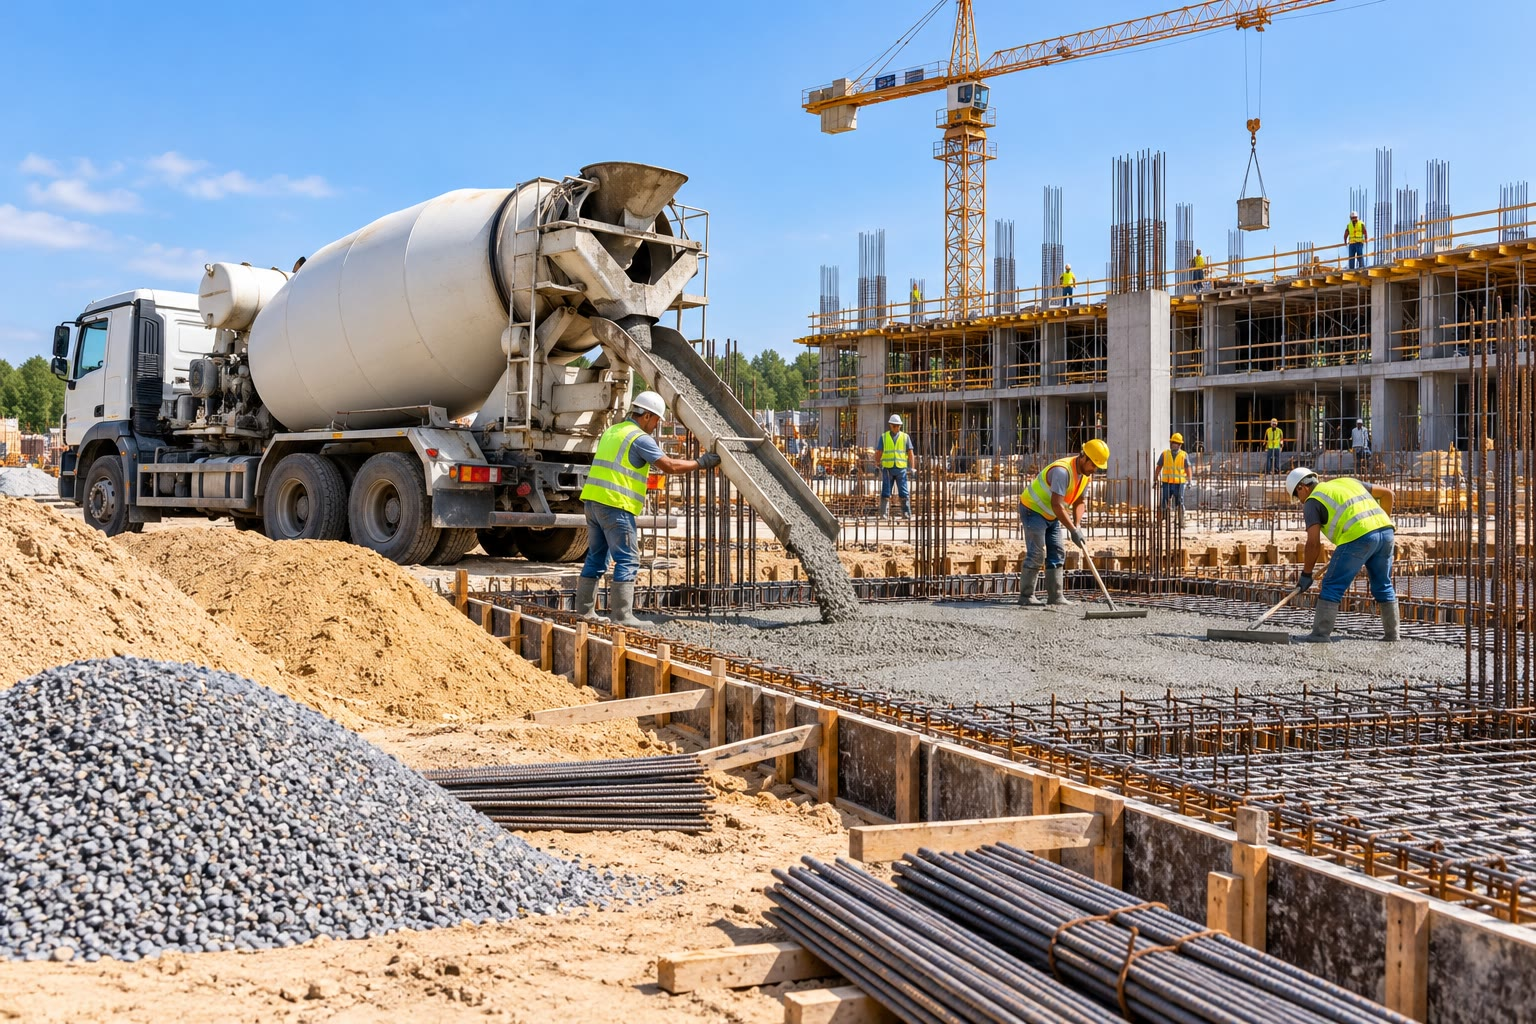
\includegraphics[width=\linewidth]{images/book1/ai/g9-building-site.jpg}
\end{minipage}\hfill
\begin{minipage}[c]{0.5\linewidth}\raggedright
{\small Os \omterm{def:g9:earth-resources:aggregate}{agregados} em ação: montes de \omterm{def:g3:stones-pebbles-sand:sand}{areia} e de \omterm{def:g3:stones-pebbles-sand:pebble}{cascalho} ao lado de um
caminhão betoneira que despeja o piso de um prédio novo (ilustração
gerada por IA de uma cena genérica).}
\end{minipage}
\label{fig:g9:earth-resources:building-site}
\end{omfigure}

\section{Renovável ou finito?}

Um recurso que a natureza renova no tempo de uma vida humana, como a água
de um \omterm{def:g6:water-underground:aquifer}{aquífero} que não é bombeado demais, pode ser usado para sempre. Uma
\omterm{def:g9:earth-resources:ore-deposit}{jazida}, uma camada de carvão ou um campo de petróleo levaram milhões de
anos para se formar. Nós os usamos em algumas décadas: na nossa escala de
tempo, eles não se renovam de jeito nenhum.
% ledger: eia:coal, earle:coal

\begin{omfigure}
\begin{tikzpicture}
\begin{axis}[xmode=log, width=12.5cm, height=4.6cm, xmin=10, xmax=1e9, ymin=0.4, ymax=4.6,
  ytick=\empty, xlabel={anos (escala logarítmica)}, label style={font=\small},
  xtick={10,100,1000,1e4,1e5,1e6,1e7,1e8,1e9},
  xticklabels={$10$,$10^2$,$10^3$,$10^4$,$10^5$,$10^6$,$10^7$,$10^8$,$10^9$},
  tick label style={font=\footnotesize}, xmajorgrids, grid style={black!12}, clip=false]
\addplot[only marks, mark=|, mark size=4pt, line width=4pt, omWarm,
  error bars/.cd, x dir=plus, x explicit, error bar style={line width=4pt, omWarm}, error mark=none]
  table[x=lo_yr, y=y, x error expr=\thisrow{hi_yr}-\thisrow{lo_yr}] {figdata/out/grade-9-concentration-times.dat};
\node[anchor=west, font=\footnotesize, fill=white, inner sep=1pt] at (axis cs:1500,4) {um pântano forma uma camada grossa de plantas};
\node[anchor=east, font=\footnotesize, fill=white, inner sep=1pt] at (axis cs:6e7,3) {idade do carvão lavrado nos Estados Unidos};
\node[anchor=west, font=\footnotesize, fill=white, inner sep=1pt] at (axis cs:150,2) {Chuquicamata explorada até hoje (mais de um século)};
\node[anchor=west, font=\footnotesize, fill=white, inner sep=1pt] at (axis cs:65,1) {reservas mundiais de cobre no ritmo de lavra de 2024};
\end{axis}
\end{tikzpicture}

{\small Tempos de formação e tempos de uso, numa escala em que cada passo
é dez vezes o anterior. O carvão é cerca de um milhão de vezes mais velho
que o tempo que uma mina leva para esgotar uma \omterm{def:g9:earth-resources:ore-deposit}{jazida}.}
% ledger: earle:coal, eia:coal, earle:chuquicamata, usgs:mcs-copper (figdata/grade-9/concentration.py, part times)
\label{fig:g9:earth-resources:times}
\end{omfigure}

Quanto tempo um recurso vai durar? Os geólogos só contam o que é
conhecido e pode ser extraído.

\begin{definition}[Reserva]\label{def:g9:earth-resources:reserve}
A \emph{reserva}\index{reserva} de um recurso \omterm{def:g6:rocks-and-minerals:mineral}{mineral} é a parte das
\omterm{def:g9:earth-resources:ore-deposit}{jazidas} conhecidas que pode ser extraída com lucro, com as técnicas e os
preços do momento.
\end{definition}
% ledger: usgs:mcs-reserves

Uma \omterm{def:g9:earth-resources:reserve}{reserva} não é tudo o que há no chão. Ela cresce quando novas \omterm{def:g9:earth-resources:ore-deposit}{jazidas}
são descobertas, quando as técnicas melhoram ou quando os preços sobem, e
diminui à medida que as \omterm{def:g9:earth-resources:ore-deposit}{jazidas} são lavradas. Em 1970, as \omterm{def:g9:earth-resources:reserve}{reservas}
mundiais de cobre eram estimadas em 280~milhões de toneladas. Desde
então, cerca de 700~milhões de toneladas de cobre foram lavradas, duas
vezes e meia essa \omterm{def:g9:earth-resources:reserve}{reserva}, e mesmo assim as \omterm{def:g9:earth-resources:reserve}{reservas} de 2024 eram
estimadas em 980~milhões de toneladas.
% ledger: usgs:mcs-reserves

\begin{dated}{2025}
Em 2024, as minas do mundo produziram cerca de 23~milhões de toneladas de
cobre. Nesse ritmo, as \omterm{def:g9:earth-resources:reserve}{reservas} de 980~milhões de toneladas durariam
$980 \div 23
\approx 43$ anos. Esse número não é uma data em que o cobre vai acabar: é
uma medida do cobre que é conhecido e que vale a pena extrair hoje.
\end{dated}
% ledger: usgs:mcs-copper (figdata/grade-9/concentration.py: 42.6 years)

Um metal, ao contrário do carvão ou do petróleo, não é destruído quando
é usado: a reciclagem dos materiais, vista nos livros de química, o
devolve. O cobre de um cabo velho, de um motor sucateado ou das sobras de
uma fábrica pode ser fundido e refinado de novo. Nos Estados Unidos, em
2024, o cobre recuperado da sucata representou cerca de \qty{35}{\%} de
todo o cobre usado.
% ledger: usgs:mcs-copper-scrap

\begin{omfigure}
\begin{tikzpicture}[font=\footnotesize, node distance=1.2cm,
  box/.style={draw=black!60, fill=black!4, rounded corners=2pt, align=center, minimum height=0.9cm, inner sep=3pt},
  flow/.style={-{Stealth[length=2.2mm]}, line width=0.9pt, black!70}]
  \node[box, fill=omWarm!12] (ore) at (0,0) {jazida\\(rocha com \qty{0.5}{\%}\\de cobre)};
  \node[box] (metal) at (4.2,0) {cobre metálico};
  \node[box] (things) at (8.2,0) {cabos, canos,\\motores};
  \node[box, fill=blue!8] (scrap) at (6.2,-2.1) {sucata};
  \node[box, fill=black!12] (waste) at (0,-2.1) {rocha triturada\\que sobra};
  \draw[flow] (ore) -- node[above] {extrair,} node[below] {concentrar} (metal);
  \draw[flow] (metal) -- node[above] {fabricar} (things);
  \draw[flow] (things) |- node[pos=0.25, right] {jogado fora} (scrap);
  \draw[flow] (scrap) -| node[pos=0.75, left] {fundir, refinar} (metal);
  \draw[flow] (ore) -- (waste);
\end{tikzpicture}

{\small Dois caminhos até o cobre metálico: a partir de um minério, com
toneladas de \omterm{def:g3:stones-pebbles-sand:rock}{rocha} escavadas e trituradas, ou a partir da sucata, que é
fundida e refinada de novo.}
\end{omfigure}

\begin{example}[A rocha que a reciclagem poupa]\label{ex:g9:earth-resources:recycling}
Um minério com \qty{0.5}{\%} de cobre contém \qty{5}{kg} de cobre em cada
tonelada de \omterm{def:g3:stones-pebbles-sand:rock}{rocha}. Para fazer uma tonelada de cobre, cerca de
$1000 \div 5 = 200$ toneladas de minério têm de ser escavadas,
trituradas e tratadas, e quase tudo termina como rejeito. Cada tonelada
de cobre feita a partir da sucata deixa essas 200 toneladas de \omterm{def:g3:stones-pebbles-sand:rock}{rocha} no
chão --- e a \omterm{def:g9:earth-resources:ore-deposit}{jazida} dura mais.
% ledger: perkins:ore-grades (computed)
\end{example}


\section{Exercícios}

\begin{exercise}[$\star$]\label{exo:g9:earth-resources:1}
Complete com a palavra certa (\omterm{def:g9:earth-resources:ore-deposit}{jazida}, \omterm{def:g9:earth-resources:ore-deposit}{fator de concentração}, \omterm{def:g9:earth-resources:aggregate}{agregado},
\omterm{def:g9:earth-resources:reserve}{reserva}). (a) A \omterm{def:g3:stones-pebbles-sand:sand}{areia} usada no concreto é um \ldots\ (b) A parte do cobre
conhecido que pode ser extraída com lucro hoje é a \ldots\ de cobre. (c)
Uma \omterm{def:g3:stones-pebbles-sand:rock}{rocha} em que um metal é rico o bastante para ser lavrado é uma
\ldots\ (d) O número de vezes que um metal foi concentrado é o seu \ldots
\end{exercise}

\begin{exercise}[$\star$]\label{exo:g9:earth-resources:2}
% ledger: earle:magmatic, usgs:gold-lode, usgs:gold-placer
Que maneira de concentrar um metal cada frase descreve: no \omterm{def:g7:volcanoes:magma}{magma}, nas
fendas pela água quente, ou nos \omterm{def:g3:stones-pebbles-sand:pebble}{cascalhos} dos \omterm{def:g1:landscapes-around-us:water}{rios}? (a) Pepitas de ouro
estão sobre a \omterm{def:g3:stones-pebbles-sand:rock}{rocha} de base, embaixo do \omterm{def:g3:stones-pebbles-sand:pebble}{cascalho} de um riacho. (b) A água
quente enche uma fenda de quartzo e ouro. (c) Uma camada de \omterm{def:g6:rocks-and-minerals:mineral}{minerais}
pesados de níquel fica no fundo de um antigo corpo de \omterm{def:g7:volcanoes:magma}{magma}. (d) O ouro
é liberado de um veio pela \omterm{def:g5:water-shapes-the-land:erosion}{erosão}.
\end{exercise}

\begin{exercise}[$\star$]\label{exo:g9:earth-resources:3}
% ledger: earle:coal, eia:coal
Ponha estas etapas em ordem: (a) a camada de plantas é enterrada sob a
\omterm{def:g3:stones-pebbles-sand:sand}{areia} de um \omterm{def:g1:landscapes-around-us:water}{rio}; (b) árvores crescem num pântano; (c) um carvão preto e
duro se forma a quilômetros de profundidade; (d) plantas mortas se
acumulam na água parada; (e) um carvão marrom e macio se forma.
\end{exercise}

\begin{exercise}[$\star$]\label{exo:g9:earth-resources:4}
Na escala de uma vida humana, cada recurso é renovável ou não? Explique
em uma frase. (a) O carvão. (b) A água de um \omterm{def:g6:water-underground:aquifer}{aquífero} bombeado menos do
que a \omterm{def:g4:clouds-rain-snow:precipitation}{chuva} o reabastece. (c) O minério de cobre. (d) O mesmo \omterm{def:g6:water-underground:aquifer}{aquífero}
bombeado duas vezes mais depressa do que é reabastecido.
\end{exercise}

\begin{exercise}[$\star\star$]\label{exo:g9:earth-resources:5}
% ledger: perkins:ore-grades
Calcule o \omterm{def:g9:earth-resources:ore-deposit}{fator de concentração} e depois escreva-o como uma potência de
dez, arredondada: (a) zinco, \qty{0.007}{\%} na \omterm{def:g6:inside-the-earth:layers}{crosta}, minério a partir
de \qty{4}{\%}; (b) estanho, \qty{0.0002}{\%} na \omterm{def:g6:inside-the-earth:layers}{crosta}, minério a partir
de \qty{0.5}{\%}; (c) ferro, \qty{5.6}{\%} na \omterm{def:g6:inside-the-earth:layers}{crosta}, minério a partir de
\qty{20}{\%}. (d) Por que o ferro precisa de tão pouca concentração?
\end{exercise}

\begin{exercise}[$\star\star$]\label{exo:g9:earth-resources:6}
% ledger: usgs:gold-placer
O ouro puro tem uma densidade de cerca de \qty{19.3}{g/cm^3}; a \omterm{def:g3:stones-pebbles-sand:rock}{rocha}
comum, de cerca de \qty{2.5}{g/cm^3}. (a) Quantas vezes o ouro é mais
denso? (b) Qual é a massa de um grão de ouro de \qty{0.01}{cm^3}, e a de
um grão de \omterm{def:g3:stones-pebbles-sand:rock}{rocha} do mesmo tamanho? (c) Explique por que, numa cheia, o
ouro acaba no fundo do \omterm{def:g3:stones-pebbles-sand:pebble}{cascalho}, sobre a \omterm{def:g3:stones-pebbles-sand:rock}{rocha} de base.
\end{exercise}

\begin{exercise}[$\star\star$]\label{exo:g9:earth-resources:7}
% ledger: perkins:ore-grades, earle:ore-grades (figdata/grade-9/concentration.py)
Use o gráfico dos \omterm{def:g9:earth-resources:ore-deposit}{fatores de concentração}. (a) Quais metais precisam de
um fator de mais de $10^3$? (b) Entre quais potências de dez fica o
cobre? (c) Quantas vezes mais o cromo precisa ser concentrado do que o
alumínio? (d) Qual dos sete metais você esperaria encontrar lavrado no
menor número de lugares? Explique.
\end{exercise}

\begin{exercise}[$\star\star$]\label{exo:g9:earth-resources:8}
% ledger: tos:sand
O mundo precisa de cerca de \qty{18}{kg} de \omterm{def:g3:stones-pebbles-sand:sand}{areia} e \omterm{def:g3:stones-pebbles-sand:pebble}{cascalho} por pessoa e
por dia. (a) Quanto é isso por pessoa em um ano, em toneladas? (b)
Escreva 50 bilhões de toneladas em notação científica. (c) Um caminhão
leva \qty{25}{t}. Quantos dias leva para a parte de uma pessoa enchê-lo?
(d) Por que tirar \omterm{def:g3:stones-pebbles-sand:sand}{areia} de um \omterm{def:g1:landscapes-around-us:water}{rio} pode fazer encolher uma praia \omterm{def:g1:landscapes-around-us:water}{rio}
abaixo?
\end{exercise}

\begin{exercise}[$\star\star$]\label{exo:g9:earth-resources:9}
% ledger: earle:oil-gas, eia:oil
(a) De que seres vivos vem a maior parte do petróleo e do gás? (b)
Abaixo de cerca de \qty{2}{km}, a que temperaturas o petróleo se forma?
(c) Por que o petróleo e o gás sobem através das \omterm{def:g3:stones-pebbles-sand:rock}{rochas}? (d) Que tipo de
\omterm{def:g3:stones-pebbles-sand:rock}{rocha} os detém, e onde eles se acumulam?
\end{exercise}

\begin{exercise}[$\star\star$]\label{exo:g9:earth-resources:10}
% ledger: earle:chuquicamata
A mina de Chuquicamata produziu mais de 29~milhões de toneladas de cobre
em mais de 100 anos. (a) Escreva 29~milhões de toneladas em notação
científica. (b) Mais ou menos, qual é a produção média por ano? (c) Se o
minério tivesse \qty{1}{\%} de cobre, quantas toneladas de minério foram
escavadas para obter 29~milhões de toneladas de cobre? Use a notação
científica. (d) Por que uma mina de um minério tão pobre tem de ser tão
grande?
\end{exercise}

\begin{exercise}[$\star\star\star$]\label{exo:g9:earth-resources:11}
% ledger: usgs:mcs-reserves, usgs:mcs-copper
Em 1970, as \omterm{def:g9:earth-resources:reserve}{reservas} mundiais de cobre eram estimadas em 280~milhões de
toneladas. De 1970 a 2024, cerca de 697~milhões de toneladas foram
lavradas, e as \omterm{def:g9:earth-resources:reserve}{reservas} de 2024 eram de 980~milhões de toneladas, com
23~milhões de toneladas lavradas em 2024. (a) Se a \omterm{def:g9:earth-resources:reserve}{reserva} de 1970 fosse
todo o cobre que existia, quando ela teria acabado? Compare com o que foi
lavrado. (b) Quantas vezes a \omterm{def:g9:earth-resources:reserve}{reserva} de 2024 é maior que a de 1970? (c)
Calcule quantos anos a \omterm{def:g9:earth-resources:reserve}{reserva} de 2024 duraria no ritmo de 2024. (d) Dê
duas razões pelas quais uma \omterm{def:g9:earth-resources:reserve}{reserva} pode crescer mesmo enquanto é
lavrada.
\end{exercise}

\begin{exercise}[$\star\star\star$]\label{exo:g9:earth-resources:12}
% ledger: earle:coal, eia:coal
Uma camada de carvão tem $3 \times 10^8$ anos. O seu pântano durou
$2 \times 10^3$ anos, e a camada é esgotada em 50 anos. (a) Escreva 50
anos em notação científica. (b) Quantas vezes mais do que a lavra durou
o pântano? (c) Quantas vezes mais velha do que o tempo da lavra é a
camada? (d) Use esses números para explicar por que o carvão é chamado
de recurso não renovável.
\end{exercise}

\section{Problema: Concreto para uma nova cidade}

\begin{problem}[{Problema de fim de semana --- uma nova cidade é
construída com a areia de uma cava local; a resposta final é o número de
anos que a reserva de areia da cava duraria}]
\label{pb:g9:earth-resources:1}
% ledger: usgs:aggregate (about 100 and 300 t per home), tos:sand (figdata/grade-9/concentration.py, part problem: exercise data)
Uma nova cidade de \num{2000} moradias vai ser construída em dez anos,
perto de uma antiga cava de \omterm{def:g3:stones-pebbles-sand:sand}{areia} escavada nos \omterm{def:g3:stones-pebbles-sand:pebble}{cascalhos} de um terraço de
\omterm{def:g1:landscapes-around-us:water}{rio}. Contando a sua parte das ruas, das escolas e das lojas, cada moradia
precisa de cerca de \qty{300}{t} de \omterm{def:g9:earth-resources:aggregate}{agregados}, dos quais \qty{40}{\%}
são \omterm{def:g3:stones-pebbles-sand:sand}{areia}. A camada de \omterm{def:g3:stones-pebbles-sand:sand}{areia} da cava tem \qty{1.2}{km} de comprimento,
\qty{500}{m} de largura e \qty{5}{m} de espessura; um metro cúbico da sua
\omterm{def:g3:stones-pebbles-sand:sand}{areia} tem uma massa de \qty{1.6}{t}. A cava também vende \num{136000}
toneladas de \omterm{def:g3:stones-pebbles-sand:sand}{areia} por ano para o resto da região.

\noindent\textbf{Parte I --- Quanta areia?}\par\nopagebreak
\begin{enumerate}[beginpenalty=10000]
  \item Uma casa de família sozinha precisa de cerca de \qty{100}{t} de
        \omterm{def:g9:earth-resources:aggregate}{agregados}. Escreva essa massa em quilogramas, em notação
        científica.
  \item Quantas toneladas de \omterm{def:g9:earth-resources:aggregate}{agregados} a cidade inteira vai precisar?
  \item Quantas toneladas isso dá por ano, ao longo dos dez anos?
  \item De quantas toneladas de \omterm{def:g3:stones-pebbles-sand:sand}{areia} por ano a cidade precisa?
\end{enumerate}

\noindent\textbf{Parte II --- A reserva.}\par\nopagebreak
\begin{enumerate}[resume, beginpenalty=10000]
  \item Calcule o volume da camada de \omterm{def:g3:stones-pebbles-sand:sand}{areia}, em metros cúbicos, em
        notação científica.
  \item Um terço da camada fica embaixo de uma vila e de uma estrada e
        não vai ser escavado. Que volume pode ser extraído?
  \item Qual é a massa dessa \omterm{def:g9:earth-resources:reserve}{reserva}, em toneladas?
  \item Quantas toneladas de \omterm{def:g3:stones-pebbles-sand:sand}{areia} a cava vai vender por ano, para a
        cidade e para a região juntas?
\end{enumerate}

\noindent\textbf{Parte III --- Renovável ou não?}\par\nopagebreak
\begin{enumerate}[resume, beginpenalty=10000]
  \item Todo ano, o \omterm{def:g1:landscapes-around-us:water}{rio} traz cerca de \num{2000} toneladas de \omterm{def:g3:stones-pebbles-sand:sand}{areia} nova
        para a área. Quantas vezes mais \omterm{def:g3:stones-pebbles-sand:sand}{areia} a cava vende?
  \item Na escala da vida da cidade, essa \omterm{def:g3:stones-pebbles-sand:sand}{areia} é um recurso renovável?
        Explique.
  \item Se a cidade substituísse um quarto da sua \omterm{def:g3:stones-pebbles-sand:sand}{areia} por concreto
        velho triturado, quantas toneladas de \omterm{def:g3:stones-pebbles-sand:sand}{areia} ela pouparia por ano?
  \item Sem essa reciclagem, quantos anos duraria a \omterm{def:g9:earth-resources:reserve}{reserva} de \omterm{def:g3:stones-pebbles-sand:sand}{areia} da
        cava?
\end{enumerate}
\end{problem}
